\chapter{Introduction}
Embedded systems \parencite{leveson_embedded_2003} are special-purpose computer systems---composed of a processor, memory, software, and peripherals for input and ouput---that are embedded into a larger mechanical or electronic system.
Embedded systems are different from general-purpose computers such as desktops, laptops, mobile phones, and tablets because they typically run a single program which is tightly integrated to the accompanying hardware it is embedded within.
Their function is often to control or monitor a machine, which requires their program to react in real-time to sensor information or user input.

Arduino is a popular starting point for learning embedded systems today.
According to its \href{https://www.arduino.cc/en/Guide/Introduction}{official website}, 
``Arduino is an open-source electronics platform based on easy-to-use hardware and software'' \parencite{arduino_what_2018}.
It comprises of three main elements: 
hardware boards, the most famous of which is the Arduino Uno, shown in Fig.~\ref{fig:arduino_uno};
a microcontroller programming interface (API) and libraries in the C++ programming language, known as the \emph{Arduino language};
and an integrated development environment, the Arduino IDE.
Its low price, usability, and extensive community support make it an excelent entry point for learning embedded systems and a rapid prototyping tool for experts.

\begin{figure}[t]
  %\begin{wide}
    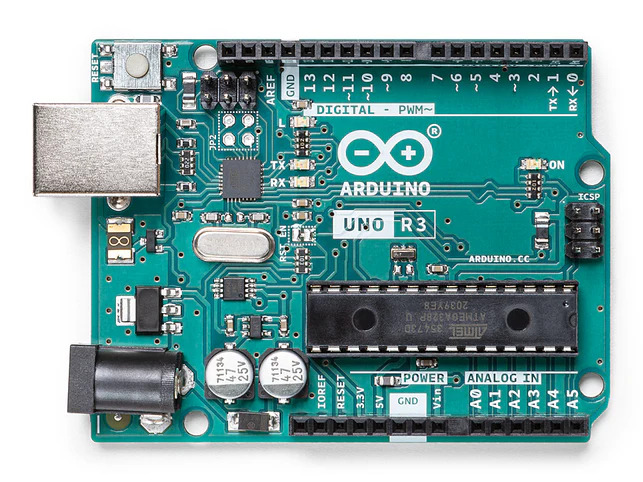
\includegraphics[width=0.5\textwidth]{img/arduino_uno_rev3}%
    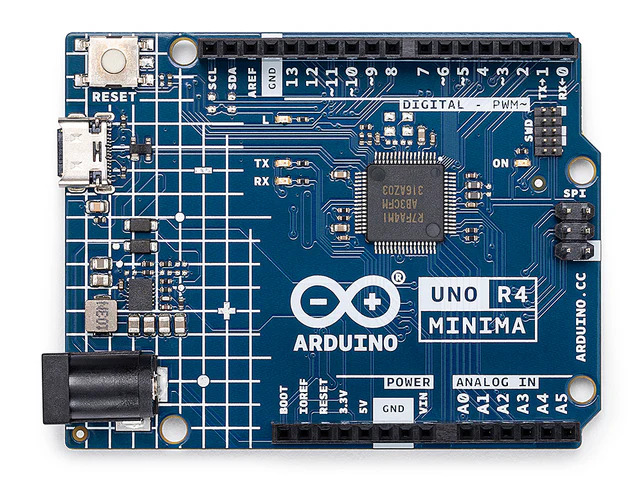
\includegraphics[width=0.5\textwidth]{img/arduino_uno_rev4}%
    \\ \scriptsize
    Source: \href{https://store.arduino.cc/collections/edu-boards}{\texttt{arduino.cc}}, under the \href{https://creativecommons.org/licenses/by-sa/3.0/legalcode}{Creative Commons Attribution ShareAlike 3.0} license.
    \caption{Arduino Uno Board Revisions Rev3 (R3) and R4 Minima.}
    \label{fig:arduino_uno}
  %\end{wide}
\end{figure}

This book is a introduction to embedded system programming with Arduino and C++.
Its main goal is laying out the foundations to understand the basic syntax of C++ and the while highlighting the unique aspects that distinguish embedded systems programming.
Its goal is enable readers to embed Arduinos or similar boards in their projects, leveraging existing libraries and frameworks instead of writing everything from scratch.
By understanding the core principles, readers will be able to integrate third-party code, modify existing solutions to fit their needs, build upon open-source projects, and even use AI in the software development process.
This approach also fosters good software engineering practices, such as code reuse, modular design, and systematic testing for robustness and correctness


\section{Platforms}
\label{sec:platforms}
A defining characteristic of embedded systems is that the software is tightly coupled to the hardware it runs on.
Because of this, it is crucial to test your code on a physical hardware board to ensure proper functionality. Fortunately, many embedded platforms are affordable and widely available, making it easy to acquire a board for hands-on development.

Recommended boards for this book are:
\begin{description}
\item[Arduino Uno Rev3]
  The classic entry-level embedded platform, with many tutorials, example projects, libraries, drivers, and compatible hardware that snap in as Arduino Shields to extend its capabilities.
  The official, Arduino-branded device costs \SI{27}[\$]{} but, as its hardware design is open, fully compatible clones can be found for as low as \SI{8}[\$]{}.
  With only \SI{2}{KB} of RAM, it is resouce-constrained yet can still drive truly impressive projects.
  It is also a very forgiving board, robust against short-circuiting its pins, slight overvoltage, and general mishandling.
\item[Arduino UNO R4]
  A cheaper (\SI{20}[\$]{}) and more capable version of the Rev3, the UNO R4 has better performance and more features while maintaining the same form factor and voltage levels.
  It offers improved processing power, more memory, and additional peripherals, making it suitable for a broader range of projects.
  An excellent choice if you need more capability than the Rev3 but still prefer to stick with the familiar Arduino environment.
  A wireless version with Wi-Fi and bluetooth is also available for \SI{27.50}[\$]{}.
\item[ESP32]
  A family of low-cost platforms, starting at below \SI{5}[\$]{}, that offer a lot of performance.
  All boards feature built-in wireless communication (Wi-Fi and Bluetooth) and dual-core processors.
  The ESP32 is a great choice for projects involving connectivity or real-time processing.
  It can be programmed in C/C++, Python, Lua, and other languages.
\item[Raspberry Pi Pico 2]
  A highly capable option, starting at around \SI{5}[\$]{}, with dual-core ARM architecture and ample memory.
  Offers wireless capabilities in some variants and is compatible with both C++ and MicroPython, making it suitable for a variety of coding environments.
  The Raspberry Pi Pico is particularly beneficial for users who want a small, affordable board with substantial memory and processing power.
\end{description}

Simulation can also be a valuable tool, especially in the early stages of development or when hardware is not immediately accessible.
Simulators allow you to prototype, debug, and test code without the need for physical deployment, though they may not always capture the full range of hardware interactions.
They are also often used in automated testing and continuous integration (CI), allowing developers to catch and fix bugs early.

Recommended simulation environments for this book are:
\begin{description}
\item[Wokwi] 
  An extensible online digital electronics simulator that runs for free on a web browser.
  Wokwi can simulate Arduino, ESP32, STM32, and Raspberry Pi Pico.
  It can simulate multiple external hardware boards and the simulated IoT devices can connect to the internet.
  The supported programming languages include C/C++, Python, and Rust.
  Wokwi does not support analog simulation, however.\\
  \url{https://wokwi.com}
\item[TinkerCad Circuits] 
  A simple, introductory Arduino simulator that has some analog simulation capabilities.
  It runs on a web browser and has some external hardware boards implemented.\\
  \url{https://www.tinkercad.com/circuits}
\end{description}

Most examples in this book can be done either in a hardware board or in simulation.
For best learning, however, familiarity with hardware is important.
Having a physical board on hand is also essential for using what you learn in personal, academic, and professional projects, beyond the book examples, which is the ultimate goal of the book.

\section{Hello World on the Wokwi Simulator}

Hello World is the first program we will see on the Arduino to introduce the structure of the code and how to send information from the Arduino to a development computer.
The program, \texttt{HelloWorld.ino} is shown in the code listing below and in Fig.~\ref{fig:wokwi-hello}, which also has a \href{https://wokwi.com/projects/420387835399008257}{link for opening it on the Wokwi simulator}.

\inofile{HelloWorld.ino}

\begin{figure}[t]
  \begin{wide}
    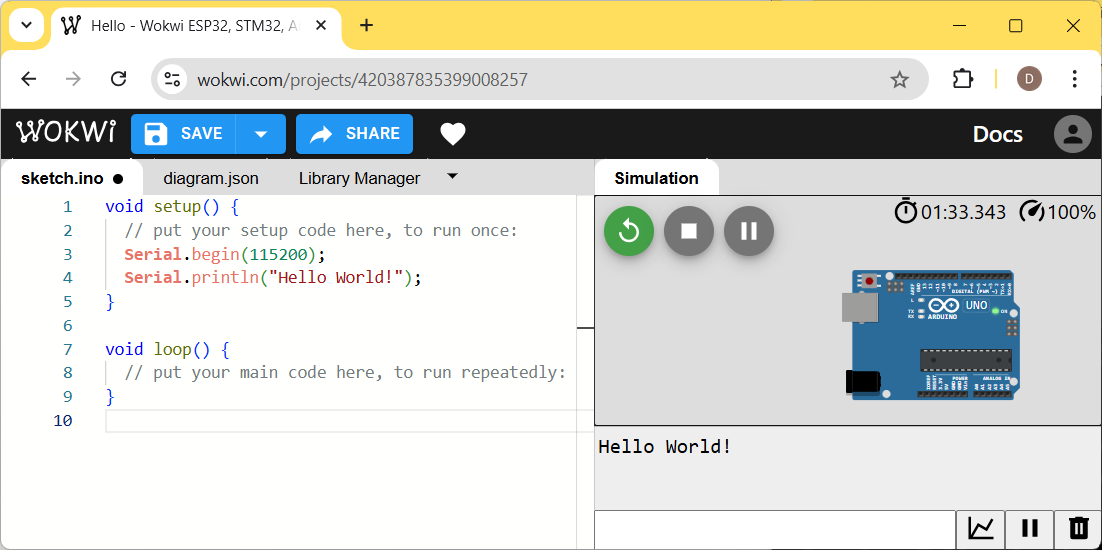
\includegraphics[width=\textwidth]{img/wokwi-hello.png}
    \\ \scriptsize
    Access this on \url{https://wokwi.com/projects/420387835399008257}
    \pending{Update this for the hello again.}
    \caption{Hello World program on the Wokwi simulator.}
    \label{fig:wokwi-hello}
  \end{wide}
\end{figure}

The program has two main blocks: the \texttt{setup} and \texttt{loop} functions.
Each function consists of the statements, or lines of code, between the curly braces \texttt{\{\}} that follow the function name.
In the code of Fig.~\ref{fig:wokwi-hello}, the \texttt{setup} function is in lines 1--5 and the \texttt{loop} function, between lines 7--9, is empty.
All the text after the characters \texttt{//}, which is typeset in grey, are comments and have no effect in the program's logic.

The Arduino program starts by executing the \texttt{setup} function which, as the name implies, usually initializes the device.
It then executes the \texttt{loop} function, which usually contains the main program logic, in an infinite loop, until the device is powered off.
Once the statements in the \texttt{loop} function are executed, it is executed again, again, and again, forever.

The microcontroller connects to the other devices by changing the voltage levels on its pins.
Some of the pins are controlled by electronics to change the voltages according to standard communication protocols.
One of these protocols is the serial communication, which consists of sending information in series (sequence) of high and low voltages, using a single pin for transmitting and another one for receiving information.
The Arduino Uno uses pins 0 and 1 for serial communication, which can be seen in Fig.~\ref{fig:arduino_uno}, labeled TX (transmit) and RX (receive).
The serial port is how the Arduino Uno Rev3 receives its programs from the development computer and is commonly used to monitor or debug the program.
In the Uno Rev3, a USB/Serial converter bridges messages between the computer's USB port and the microcontroller's serial port.

Serial communication requires both parties to agree on the rate the symbols are sent, since they are sent in sequence on the same pin.
This is important for both parties to correctly decode the voltages on the line as bits of data.
In the example code, this is done at line 3, in the \texttt{setup} function, where the statement \inocodei{Serial.begin(115200)} sets the rate at \SI{115200}{baud}, that is, \num{115200} symbols per second.
In an Arduino program, the serial port has to be explicitly configured with a baud rate before it is used to transceive data.

The next line of the program sends (prints) the text ``Hello World!'' followed by a line return, which moves the cursor to the next line.
To run the program on the simulator, click on the green \emph{Start the simulation} button under the \emph{Simulation} tab.
This will bring up the Serial Monitor pane, on which the text sent over the serial port is printed.
As the \texttt{loop} function of this example program is empty, the microcontroller does nothing after the \texttt{setup} function is over.

\section{Hello World on the Hardware Board}

The same example can be run on a hardware board, using the Arduino IDE to program the board and monitor its response.
All that needs to be done is an extra step in selecting the board and its communication interface.
\pending{Update this, a lot of extra steps actually are needed if you are a beginner.
Saying it is very simple gives a bad message to people who struggle.}

\subsection{Install the Arduino IDE}
If you haven't done so, install the Arduino IDE from its official website%
\footnote{Downloads links can be accessed directly at \url{https://www.arduino.cc/en/software}}
\texttt{\href{https://www.arduino.cc/en/software}{arduino.cc}}.
Note that the Arduino IDE is free, open-source software, but the software download links push users to donate to the Arduino Foundation and subscribe to a Newsletter.
I recommend downloading the software first and trying it out before making a donation or subscribing, for that simply click on the link that says \emph{just download}, right below the highlighted buttons for donating or subscribing.

I strongly recommend using the IDE version 2 or higher, as version 1.x lacks line numbers and cannot handle  well the large number of boards and libraries that exist today.
For Windows users, if using the Microsoft Store, make sure you install \emph{Arduino IDE 2} by Arduino LLC, and not \emph{Arduino IDE}, which is version 1.8.

\subsection{Install Board Support}
If you are using a board other than the Uno Rev3, you must install the board support, which contains the compiler and development tools for uploading code to the microcontroller.
To do that, open the \emph{Boards Manager} in the Arduino IDE, either by selecting the icon in the left toolbar, as shown in Fig.~\ref{fig:ide-2-overview} or in the menu \emph{Tools $\to$ Board $\to$ Boards Manager}.
For each of the platforms mentioned in Sec.~\ref{sec:platforms}, install the following board:
\begin{description}
\item[Arduino Uno Rev3] Arduino AVR Boards by Arduino, should come preinstalled with the IDE.
\item[Arduino UNO R4] Arduino UNO R4 Boards by Arduino.
\item[ESP32] esp32 by Espressif Systems.
\item[Raspberry Pi Pico] Arduino Mbed OS RP2040 Boards by Arduino.
\end{description}

During installation of the board support package, you may be prompted to install the driver of your board.
These are necessary for the computer to be able to communicate with the device appropriately.
If the driver is not properly installed, it might not show up on the board selector.
Refer to the Arduino help center for more detailed, up-to-date instructions on how to add boards to the Arduino IDE%
\footnote{\url{https://support.arduino.cc/hc/en-us/articles/360016119519}}.

\begin{figure}[b]
  \begin{wide}
    \centering
    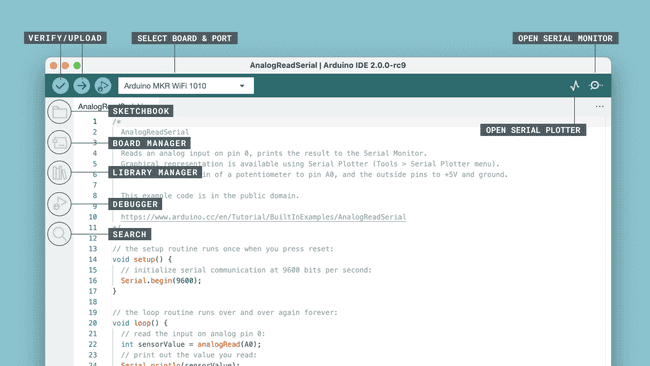
\includegraphics[width=\textwidth]{img/ide-2-overview}%
    \\ \scriptsize
    \raggedright
    Source: \href{https://docs.arduino.cc/software/ide-v2/tutorials/getting-started-ide-v2/}{\texttt{arduino.cc}}, under the \href{https://creativecommons.org/licenses/by-sa/3.0/legalcode}{Creative Commons Attribution ShareAlike 3.0} license.
  \caption{Overview of the most commonly used tools of the Arduino IDE 2.
    \pending{Remove extra stuff from this image, perhaps ask chatgpt to make blue background transparent, remove unneeded space from the bottom showing some random program.}
  }
  \label{fig:ide-2-overview}
  \end{wide}
\end{figure}

\subsection{Selecting the Board and Uploading}
Next, open the Arduino IDE and connect your board to one of your computer's USB ports.
An LED in the board should light up, indicating it is powered up.
On the top toolbar of the IDE, as shown in Fig.~\ref{fig:ide-2-overview}, the board and port can be selected.
The board and port can also be chosen in the \emph{Tools} menu.
Refer to the Arduino help center for more detailed, up-to-date instructions on how to select the board and port in the Arduino IDE%
\footnote{\url{https://support.arduino.cc/hc/en-us/articles/4406856349970}}.
If you cannot find your board, then the board support is not installed correctly.
If you cannot find the port, usually either the driver was not installed correctly or there is some problem with the board.

\begin{figure}[b]
  \centering
  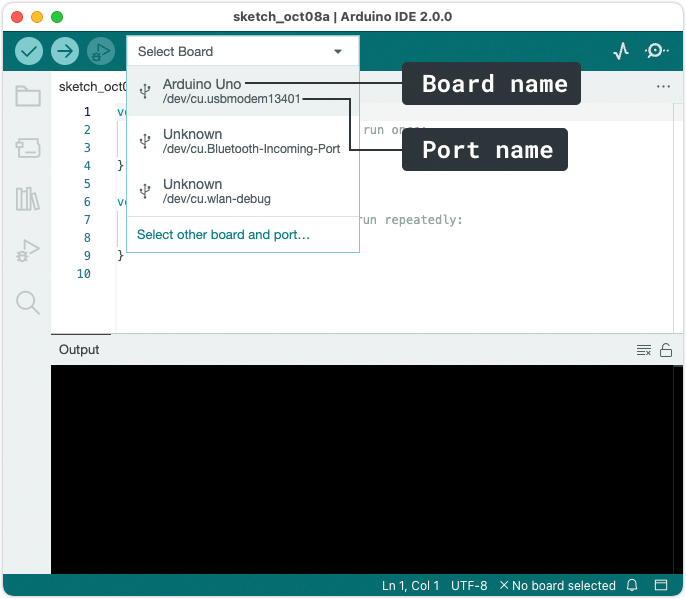
\includegraphics[width=\textwidth]{img/board-selector-labels}%
  \\ \scriptsize
  \raggedright
  Source: \href{https://support.arduino.cc/hc/en-us/articles/4406856349970-Select-board-and-port-in-Arduino-IDE}{\texttt{arduino.cc}}, under the \href{https://creativecommons.org/licenses/by-sa/3.0/legalcode}{Creative Commons Attribution ShareAlike 3.0} license.
  \caption{Board and port selection tool of the the Arduino IDE 2.
    \pending{This image is too large.}
  }
  \label{fig:board-selector-labels}
\end{figure}

After the board is selected, type the program \texttt{HelloWorld.ino} or copy the file from the book source code repository.
Then, compile and upload the code by clicking on the \emph{Upload} button on the top toolbar, shown in Fig.~\ref{fig:ide-2-overview}.
The \emph{Output} panel should open in the bottom of the IDE and some compilation messages displayed.
The board's LEDs named RX and TX should blink momentarily while the program is tranfered to the board and a message will be displayed at the bottom of the IDE when the process is concluded.
\pending{Check what message is displayed. Get a screenshot.}
\pending{Create repository.}
\pending{Create link for code listing in document.}
\pending{Number code listings.}

\subsection{Viewing the Program Output}
After the program is uploaded, the board is reset and the program starts executing.
\pending{Question: how do I stop it from running?}

\pending{Summary of what needs to be done.}
\begin{enumerate}
\item Open the Serial Monitor.
\item Select the baud rate.
\item Reset.
\end{enumerate}

%%% Local Variables:
%%% TeX-master: "main"
%%% eval: (adaptive-wrap-prefix-mode t)
%%% eval: (visual-line-mode t)
%%% eval: (nlinum-mode t)
%%% TeX-engine: luatex
%%% End:
